\documentclass{article}
    \usepackage[margin=0.7in]{geometry}
    \usepackage[parfill]{parskip}
    \usepackage[utf8]{inputenc}
    \usepackage{physics}
    \usepackage{amsmath,amssymb,amsfonts,amsthm}
    \usepackage{graphicx,wrapfig}
    \usepackage{enumitem}
    \usepackage{natbib}
    \usepackage{caption}
	\bibliographystyle{abbrvnat}
	\usepackage{hyperref}
	\hypersetup{
    colorlinks=true,
    linkcolor=blue,
    filecolor=magenta,      
    urlcolor=cyan,
    pdftitle={Overleaf Example},
    pdfpagemode=FullScreen,}

    \newcommand\ion[2]{#1$\;${\scshape{#2}}}%    
    \newcommand{\Dsh}{\rotatebox[origin=c]{180}{$\Lsh$}} 

\begin{document}
\section*{CLEDB - CORONAL FIELD DATABASE INVERSION \\ ALGORITHM NOTES}

\textbf{Contact:} Alin Paraschiv arparaschiv@nso.edu, paraschiv.alinrazvan+cledb@gmail.com

~

~

\textbf{Purpose:\\} 
Describe the main algorithm concepts, functions, and variables, comprising the CLEDB inversion algorithm for coronal magnetic fields.

~

\textbf{Main synopsis:\\} 
The aim is to invert coronal magnetic field information from observations of polarized light. The algorithm takes arrays of one or two sets of Spectroscopic Stokes IQUV observations [sobs\_in] along with their header information. The data and metadata are pre-processed, and optimal corresponding sets of databases are selected and read from disk storage. 

The data analysis is split into two branches, based on the available polarized coronal Stokes observations: 
\begin{itemize}
\item \textbf{1-line branch:} 4 input IQUV observations (one coronal emission line).
\item \textbf{2-line branch:} 8 input I$_1$Q$_1$U$_1$V$_1$I$_2$Q$_2$U$_2$V$_2$ observations (two coronal emission lines).
\end{itemize} 

Spectroscopic analysis products are computed for both 1-line or 2-line branches.

The 1-line branch employs analytical approximations to calculate line of sight (LOS) integrated magnetic field products, while the 2-line branch offer access to additional invertible magnetic field products. This second case benefits from more degrees of freedom allowing us to break degeneracies intrinsic in the inversion. Thus, the two-line algorithm branch uses a $\chi^2$ fitting method between the observation and a forward modeled database to recover full 3D vector magnetic field components.  

The database is generated via forward modeling of combinations of input magnetic field and geometric parameters.  Databases are not computed dynamically for each observation and are used as a static input with respect to the inversion scheme.

~

\textbf{Motivation for approach:\\}
By utilizing 2-line observations, we recover the 3D magnetic field information for single point voxels using a $\chi^2$ fitting approach. Generating forward calculation in the order of 10$^7$-10$^9$ atomic plasma and magnetic configurations are needed in order to satisfy solution resolution criteria. Forward modeling such solutions in a dynamic fashion is time consuming. Such a calculation (e.g. iterating for 1 pixel) has execution times in the order of 10 hours, on a single thread, with a fast FORTRAN implementation of CLE code. 

Building a separate database (the CLEDB\_BUILD module in our algorithm) to store a vast set of synthetic Stokes observations, along with the input plasma and magnetic field configurations responsible for producing polarized emission, proved to be a significantly more feasible approach. Additionally, the database theoretical calculations gain intrinsic access to otherwise un-observables input parameters (e.g. atomic alignment $\sigma_0^2$) that can be used to break inherent degeneracies encountered when attempting analytical inversions (as implemented in the 1-line branch). The dimensionality of the problem at hand can be further reduced by 1-2 orders of magnitude by using native symmetries when building and querying databases. More details on the physics aspects of dimensionality reduction and degeneracy breaking effects can be found in \citet{2020ApJ...889..109D,2021ApJ...912...18J}, and \citet{par2021}.

\newpage



\textbf{Inversion module overview scheme:\\} 
The algorithm is split into three parts: 
\begin{itemize} 
\item CLEDB\_BUILD - The BUILD module contains pre-configured scripts for generating a database used downstream to fit the observations. FORTRAN binaries and bash scripting is used by this module. Running the default configured "\emph{rundb\_1line.sh}" script for each line on the observation is enough in most cases. Please see the dedicated README\_RUNDB for more detailed instructions.
 
\item CLEDB\_PREPINV - The PREPINV module prepares the data for analysis and matches required databases to read(for the 2-line branch). The ctrlparams anc constants classes are imported separately and fed to the module.

\item  SPECTRO\_PROC, BLOS\_PROC, and/or CLEDB\_INVPROC are the third step data analysis modules. These perform analytical or database inversion schemes on the input observational data to recover the desired plasma and magnetic field parameters (the OUTPUTS).
\end{itemize} 

\textbf{Algorithm schematic definitions:\\} 
Below we illustrate our definitions for the flowcharts describing different algorithm operations. We note that the flowcharts are not exhaustive and are not meant to describe the code to the level of individual operations. The flowcharts list the main variables and functions used along with how they are processed by the different modules and intrinsic functions, and the resulting outputs. 



\begin{figure}[!h]
 \hspace{-0.8cm}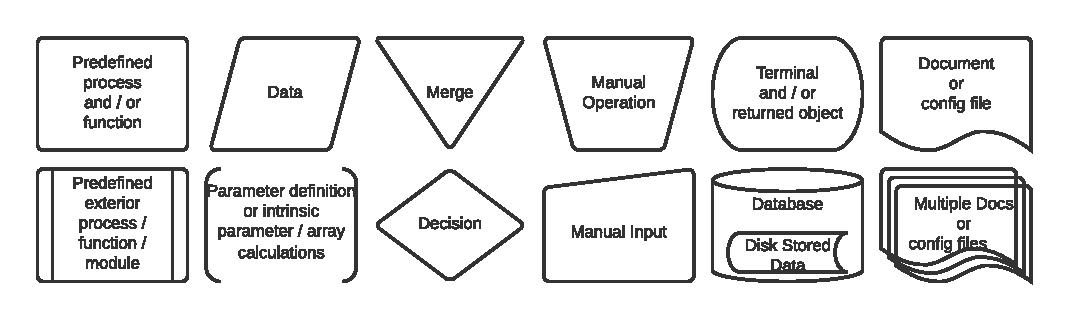
\includegraphics[width=1.08\columnwidth]{figs/shape_defs.pdf}
\end{figure} 

 Details about the modules along with the main inputs and outputs are presented in the following module schematic view. Each module is described separately in the following sections. The most important variables and defined functions are described for each inversion module component. The definitions and accompanying diagrams are not meant to be 1:1 mirrors of the coding, but merely to trace the most crucial operations and resulting outputs. Common terminology is defined in the last section. Additional extended comments can be found in each module's scripts.

\begin{figure}[!p]
\vspace{-1cm}\hspace{-2cm}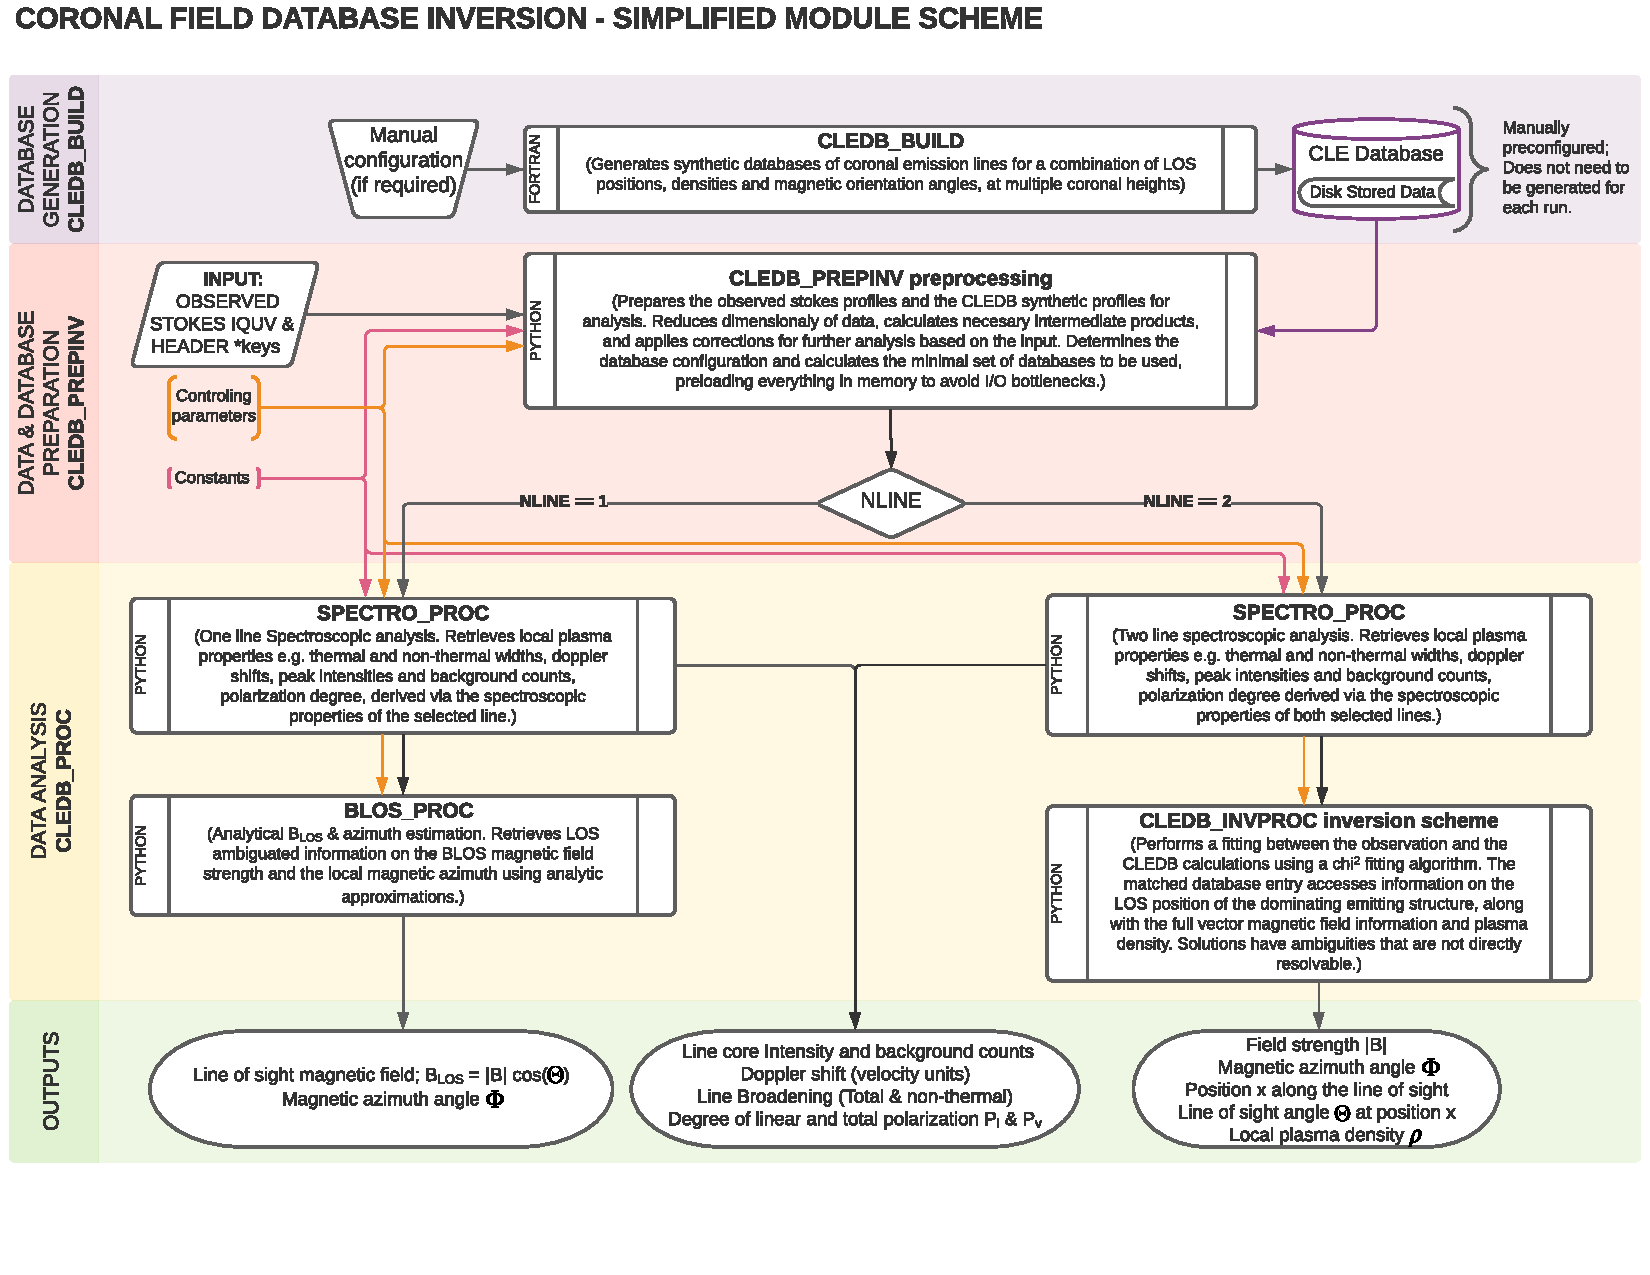
\includegraphics[angle=-90,width=1.1\columnwidth]{figs/1_CLEDB_OVERVIEW.pdf}
\end{figure} 


\newpage

\textbf{\large Instalation instructions, Python environment setup, and basic run examples:}

The CLEDB coronal field inversion code distribution is hosted on the following \href{https://github.com/arparaschiv/solar-coronal-inversion}{Github repository.} 

To create a local deployment use the git clone function:

\emph{\color{red} git clone https://github.com/arparaschiv/solar-coronal-inversion}

CLEDB\_BUILD uses precompiled GNU compatible FORTRAN binary executable files to generate databases. The module is run by utilizing a bash script that enables parallel runs of serial computations. Binaries for both Darwin and Linux architectures are provided. More details will follow in the section describing the CLEDB\_BUILD module.
Note: The FORTRAN source code is based on CLE, and not included in this package. A separate repository will be created in the near future. The source code is meant to be publicly available and can be requested from us.


The two other modules of CLEDB are written in Python. 
The Anaconda environment is utilized. Anaconda documentation and installation instructions can be \href{https://docs.continuum.io/anaconda/install/}{found here}.

We provide a configuration file, \emph{\color{red}CLEDBenv.yml} to create a custom Anaconda environment. The configuration file is used to configure the CLEDB required python packages. In a terminal session  create the environment:

\emph{\color{red}conda env create -f CLEDBenv.yml}
 
After installing all packages the environment can be activated via:

\emph{\color{red}conda activate CLEDBenv}

(The user can return to the standard python package base by running \emph{\color{red}conda deactivate}.)

The "CLEDBenv" anaconda environment installs specific version packages. Updating the python packages inside the environment is not recommended and might break functionality. If problems arise, CLEDBenv can be deleted and recreated with the default packages from the .yml.

\emph{\color{red}conda remove --name CLEDBenv --all}

Databases can be built with:

\emph{\color{red}./rundb\_1line.sh} 

See detailed database build instructions via the dedicated readme in the CLEDB\_BUILD directory.

Two examples of running the full inversion package (assuming databases are already built) are provided as Jupyter notebooks and/or lab sessions.

\emph{\color{red}jupyter-lab test\_1line.ipynb}\\
\emph{\color{red}jupyter-lab test\_2line.ipynb}

\textbf{\large External python modules:\\}
For numerical computation efficiency, the CLEDB distribution heavily relies on the Numpy and Numba packages. 
\begin{description} [font=\normalfont,leftmargin=0.6in,style=multiline]
	\item[Numpy]
Numpy provides fast vectorized operations on its self implemented-ndarray datatypes. All Python based modules are written in a Numpy-centric way. Functional equivalent pure python coding is avoided when possible due significantly slower runtimes. Numpy version specific (1.20) documentation is \href{https://numpy.org/doc/1.20/}{found here.}
	\item[Numba]
Numba implements just in time (JIT) compilation decorators and attempts to perform loop-lifting and scale serial tasks on available CPU threads. Numba has two modes of operation, object-mode and non-python mode. Non-python mode will maximize optimization and runtime speed, but is significantly limited in terms of python and/or  numpy function compatibility. The CLEDB\_PREPINV module can only be compiled in object-mode due to disk I/O operations that are not implemented in non-python mode.

A Numba enabled implementation can utilize only a small subset of Python and Numpy functions. Significant data sanitation and statically defined function input/output are required in order to enable runtime optimization and parallelization. Due to these sacrifices, coding implementations are not always clear and straightforward. Extensive documentation, python and numpy function lists, and examples can be found in the Numba documentation. The version specific (0.53.1) documentation is \href{https://numba.readthedocs.io/en/0.53.1/}{found here.}
	\item[Others]
scipy, numexpr, glob, and os are additional modules used primarily by CLEDB\_PREP for I/O operations.
	\item[]
time and sys are used during debug runs with high level of verbosity.
\end{description}


\newpage
\subsection*{CLEDB Inversion input variables and parameters:}

\textbf{A. Input data and metadata to process:}

\begin{description}
    [font=\normalfont,leftmargin=1.5in,style=multiline]
    \item[header *keys]
        Set of input header metadata information that should describe the sobs\_in list. Expected keywords with simplified naming are detailed in this section. Detailed keyword information can be found in the case of DKIST observations in the SPEC\_0214 and SPEC\_0230 reference documents.
    \item[*keys to crpixn]
        int; Reference pixel along x y or w(wavelength) direction.
    \item[*keys to crvaln]
        float; Coordinate value at crpix along x y or w(wavelength) direction.
    \item[*keys to cdeltn]
        float; Spatial (x,y) or spectral (w) platescale sampling along a direction
    \item[*keys to linpolref]
    		float, (0;2$\pi$) range; Direction of reference for the linear polarization. This is a physical convention based on the fixed orientation of a spectrograph retarder. linpolref = 0. implies the direction is corresponding to a horizontal axis, analogous to the unit circle reference. Direction is trigonometric. The units are in radians.       
    	\item[*keys to instwidth]
    		float; Measure of the utilized instrument's intrinsic line broadening coefficient. The units are in nm or km s$^-1$.  
    \item[*keys to nline]
        int; Number of targeted lines 1 $||$ 2; The inversion can accept one line or two line observations.   
    \item[*keys to tline]
        string array, [nline]; containing the name of lines to process. Naming convention follows the database directory structure described as part of the CLEDB\_BUILD module.
    \item[*keys to xs/naxis1]
         int; Pixel dimension of sobs\_in array along the horizontal spatial direction.
    \item[*keys to ys/naxis2]
         int; Pixel dimension of sobs\_in array along the vertical spatial direction.
    \item[*keys to ws]
         int; Pixel dimension of sobs\_in array along the spectral dimension.               
    \item[*keys to skybright]
    		float; sky brightness measurement used to judge observation quality and rms.
    \item[*keys to grtngba \& grtngang] 
    		float; The grating order and position; used to find central wavelength of input observation and judge suitability for inverting.   
    	\item[keyvals]
    		List; order is nx, ny, nw, nline, tline, crpix1, crpix2, crpix3, crval1, crval2, crval3, cdelt1, cdelt2, cdelt3, linpolref, instwidth;  This is a variable pack used to more easily feed the necessary parameters to other modules/functions.                        
    \item[sobs\_in]
         [2][xs,ys,ws,4] (1-line) or [2][xs,ys,ws,4] (2-line) float arrays passed as a numba typed list at input. Data are input Stokes IQUV observations of one or two lines respectively. The list will be internally reshaped as a numpy float array of [xs,ys,ws,4] or [xs,ys,ws,8] size.  
\end{description}

\textbf{B. [Control Parameters]}

Python class that unpacks control parameters used in all modules of the inversion setup. This is an editable imported module that users access and modify. The importlib module is used in the example notebooks to reload changes.

\begin{description}
    [font=\normalfont,leftmargin=1.3in,style=multiline]
	\item[dbdir]
	string; Directory where the database is stored after being built with CLEDB\_BUILD. This is the main directory, and not one of the individual ion subdirectories (e.g. fe-xiii\_1074, etc.).
	\item[reduced]
	boolean; Control parameter to reduce the database size before searching for solutions by using the linear polarization measurements. Dimensionality of db is reduced by over 1 order of magnitude and runtimes are significantly sped-up. Solution ordering might be slightly altered in certain circumstances.
	\item[nsearch]
	uint; number of solutions to compute and return for each voxel. 
	\item[gaussfit]
	uint; Variable to switch between CDF fitting and Gaussian parametric fitting with optimization.
	\item[]
	gaussfit == 0: Process the spectroscopic line parameters using only the CDF method.
	\item[]
	gaussfit == 1: Fit the line using a optimization based Gaussian procedure. This approach requires a set of 4 guesswork parameters, namely, the approximate maximum of the emission, the approximate wavelength of the core of the distribution, its standard deviation, and an offset (optional, hard-coded as 0).
	\item[]
	gaussfit == 2: Fit the line using a optimization based Gaussian procedure. In this case, the initial guesswork parameters are fed in from the results of the CDF solution, where the curve theoretically optimizes for a more accurate solution, with sub-voxel resolution.	
	
	\item[bcalc]
	uint; Method to compute the field strength in the case of 2-line observations.
	\item[]
	bcalc == 0: Use the field strength ratio of the first coronal line in the list.
	\item[]
	bcalc == 1: Use the field strength ratio of the second coronal line in the list.
	\item[]
	bcalc == 2: Use the average of field strength ratios of the two coronal lines.
	\item[maxchisq]
	float; stops searching for solutions if fitting surpassed this maxchisq threshold.
	\item[verbose]
	uint; Verbosity controlling parameter that takes vales 0-3. Levels are incremental (e.g. lev 3 includes outputs from levels 1 and 2) Due to library incompatibilities, enabling higher level verbosity will block Numba optimization of the code. 
	\item[] 
	verbose == 0: Production; silent run.
	\item[]
	verbose == 1: Debug; prints the current module and operation being run.
	\item[]
	verbose == 2: Debug; implements warnings for common caveats.
	\item[]
	verbose == 3: Debug; will enable execution timing for selected sections. Numba will fall-back to object-mode.
	\item[numbajitflag]
	boolean; Variable that controls the enabling of Numba just in time compilation (JIT) decorators. Higher level verbosity requires disabling the JIT decorators. 
\end{description}


\textbf{C. [Constants]}

        Python class that unpacks physical constants needed during the inversion. It is mainly utilized by the SPECTRO\_PROC module. Ion specific and general atomic and plasma constant parameters are stored herein. The class self-initializes for each required providing its "Ion specific" parameters in a dynamic fashion.

\begin{description}
    [font=\normalfont,leftmargin=1.3in,style=multiline]

		\item[-------------------]
		---------------------------Physical constants----------------------------------	
		\item[solar\_diam]
		float*4 variables; Solar diameter in arcsecond, degrees, radians, and steradian units.
		\item[l\_speed] 
		float; Speed of light; SI [m s$^{-1}$]  
		\item[kb]
		float; Boltzmann constant; SI [m$^2$ kg s$^{-2}$ K$^{-1}$]
		\item[e\_mass]
		float; Electron mass; SI [Kg]
		\item[e\_charge]
		float; Electron charge; SI [C]
		\item[planckconst]
		Planck's constant; SI [m$^2$ kg s$^{-1}$];
		\item[bohrmagneton]
		Bohr Magneton; Mostly SI converted to Gauss units [kg m$^2$ s$^{-2}$ G$^{-1}$]		
		
		\item[-------------------]
		---------------------------Ion specific constants--------------------------------		
		\item[ion\_temp]
		float; Ion temperature; SI [K]
		\item[ion\_mass]
		float; Ion mass; SI [Kg];   
		\item[line\_ref]
		float; Theoretical line core wavelength position; [nm]					
		\item[width\_th] 
		float; Thermal width analytical approximation; [nm]
		\item[F\_factor] 
		float; Additional factor described by \citet{2020ApJ...889..109D}. Useful in calculating LOS products;		
		\item[g$_u$ \& g$_l$] 
		float; Atomic upper and lower energy levels factors; LS coupling;
		\item[j$_u$ \& j$_l$]	
		float; Atomic upper and lower level angular momentum terms;
		\item[g$_{eff}$]
		float; LS coupling effective Land\`{e} factor;
\end{description}



\newpage
\subsection*{CLEDB\_BUILD Database Generation}

\textbf{Purpose:} The CLEDB\_BUILD module to generate a database of synthetic IQUV profiles for the four ions in question, with a range of density estimations, range of possible LOS positions, and all possible magnetic angle configurations, for one magnetic field strength B=1.  In normal circumstances this module is only run once per system where the inversion is installed. A module diagram is provided in this section.

\textbf{CLEDB\_BUILD Configuration files} (in config directory)
\begin{description}
    [font=\normalfont,leftmargin=1.3in,style=multiline]
	\item[DB.INPUT]
	Main configuration file for the database generation. It is important to keep the same number of parameter decimals and white spaces when modifying this file. The parameters are described separately below. 
    \item[ATOM.ion]
    	These files contain the atomic configuration data to be used for calculations. These are reduced level calculations that mimic the IQUV fluxes from a full level calculation in the selected infrared coronal lines. In general, users should not modify these files.
	\item[INPUT.ion(a/b)]
	These are input and configuration files that are read when generating databases. The \emph{wlmin} and \emph{wlmax} parameters control which lines described in the ATOM.ion files are outputed. In the case of Fe XIII, a separate INPUT configuration is needed for each line. In general, users should not modify these files.   
	\item[IONEQ]
	Ionization equilibrium data from CHIANTI.
	\item[GRID.DAT]
	Defines the range and resolution of a CLE simulation. In the case of database building it has a very limited functionality and is only kept due to CLE's dependency on it.
	\item[db"xxxx"\_"arch"]
	Executable binaries for generating databases. "xxxx" is the current version of the FORTRAN code. arch is "linux", "rclinux" or "darwin". The different versions are provided in the distribution for cross-platform compatibility.	
\end{description}
    
\textbf{DB.INPUT parameters}
\begin{description}
    [font=\normalfont,leftmargin=1.6in,style=multiline]
	\item[ny, ymin, ymax]
	Number of y (horizontal) heights to compute databases for, in $R_\odot$ units. The ny heights are spanned between ymin and ymax values. Regardless of user input, polarization signal is not computed for $R_\odot<$ 1 due to physics of coronal emission. The amount of circular polarization drastically decreases with height. One should not normally expect to reasonably recover circular polarization signal at y $>1.5-2R_\odot$.  
	\item[ned, elnmin, elnmax]
	Number of ambient electron density values to compute calculations for. elnmin and elnmax define a logarithmic range to spread the ned densities in. The base measurement is an analytical approximation of a standard electron density expected for a y height above the limb. For example, at y=1.1$R_\odot$ we expect a logarithm of density $\log(n_e)$ of $\sim$8 electrons. setting ned=10 and elnmin=-2 and elnmax=2 will generate databases for 10 density values logarithmically scaled between $\log(n_e)$=6 and $\log(n_e)$=10.
	\item[nx, xmin, xmax]
	Number of x (depth along the LOS) positions to compute databases for, in $R_\odot$ units. The nx positions are spanned between xmin and xmax values. Due to geometric considerations, setting xmin and xmax values to more than $\pm$1.5$R_\odot$ will most probably not result in practical benefits. 
	\item[nbphi, bpmin, bpmax]
	Number of magnetic azimuth angles to compute. The angles are spread along a 0 - 2$\pi$ range.
	\item[nbtheta, btmin, btmax]	
	Number of magnetic LOS angles to compute. The range is set to 0 - 1$\pi$ (reduced range due to spherical integration).
	\item[NOTE:]
	Due to how the problem is posed, please do not reverse the ranges between nbphi and nbtheta, as it would lead to the inversion failing.	
\end{description}

\begin{figure}[!p]
\vspace{-1.9cm}\hspace{+1.5cm}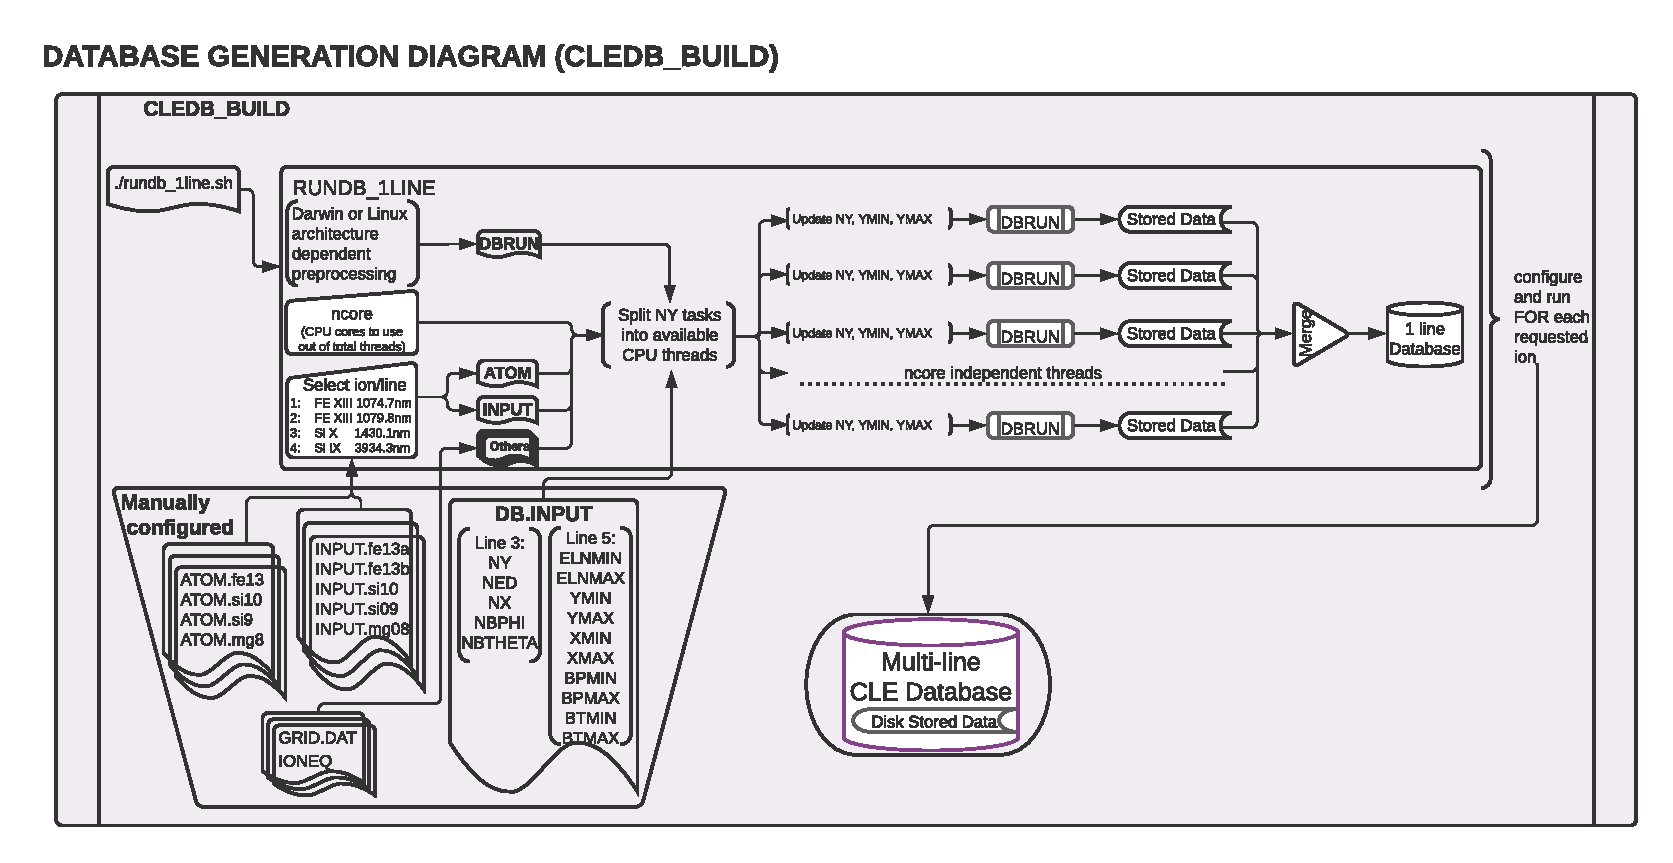
\includegraphics[angle=-90,width=0.79\columnwidth]{figs/2_CLEDB_BUILD.pdf}
\end{figure} 

\newpage

\textbf{CLEDB\_BUILD job script:}

The "{\color{red}rundb\_1line.sh}" job script will ingest the ATOM, INPUT, DB.INPUT, etc. files and split the job into available CPU threads. The user is asked for keyboard input on how many threads to use and for which line/ion to generate a database.

The script runs in a bash shell terminal session. It can handle both Linux and Darwin (OSX) environments. For OSX, an additional dependency is required. Users should install the GNU implementation of the sed command. The simplest way is to use the homebrew environment:

\emph{\color{red} brew install gnu-sed}

The job script will split the serial ny tasks on the selected CPU threads and run in dedicated folders that will be sanitized upon completion, leaving only the output database files and metadata headers. 

Logs for each script are written in real time and can be checked interactively as the job is running.

\emph{\color{red} tail BASHJOB\_"X".LOG}

Extensive notes about the parallel job script implementations are found in the additional README\_RUNDB.md file included with CLEDB\_BUILD module.

~ 

\textbf{CLEDB\_BUILD output:}

Databases for 1 to 4 of the currently available ions/lines can be constructed by running the job script successively for each.
The output database is written to the storage disk. CLEDB\_BUILD will write compressed data using a simple float64$\rightarrow$ int16 conversion using a division constant, currently set to -2.302585092994046e15. Same constant needs to be used when writing but also when reading databases into memory as part of the CLEDB\_PREPINV module.

Each individual line will be written in its dedicated folder. This database folder hierarchical system is needed in order to ingest the useful database calculations by the CLEDB\_PREPINV module. The folder system is defined as: "element-ionstage\_line". This convention is used by all modules in the CLEDB inversion distribution.
\begin{enumerate}
 \item "fe-xiii\_1074" 
 \item "fe-xiii\_1079"
 \item "si-x\_1430"
 \item "si-ix\_3934". 
\end{enumerate}
WARNING: Running successive jobs for the same ion/line will erase its database contents if they exist! 

Individual data stores for each computed y height are generated to ease I/O operations when reading data into memory. A db"xxxx".dat file is generated for each ny height, where "xxxx" represents the distance above the limb in units of $R\_\odot$. A metadata db.hdr file is produced in the individual directory that contains the dimensions and parameters applicable to any one database set of files.
 
WARNING: The user should not change the parameter configurations in DB.INPUT between multiple ion/line runs that should be part of the same database. 

Generating $\sim 5\cdot 10^8$ calculations per line for two lines will occupy $\sim$ 8 Gb of disk space.



\newpage
\subsection*{CLEDB\_PREPINV Data Pre-processing}


\textbf{Purpose:} The CLEDB\_PREVINV module processes both the input data and the database to prepare for the main inversion processing. for 1-line cases, only the observation is pre-processed. Keywords are ingested, the geometric height is computed and the spectroscopic IQUV profiles are integrated. For 2-line observations, the observation linear polarization is rotated to match the database calculation. The module then performs a match between the input data and database configuration. Only the optimal subset of database entries are pre-loaded into memory to minimize I/O operations but also to avoid I/O bottlenecks when running the fast analysis routines in the CLEDB\_PROC module. 

~

\textbf{CLEDB\_PREPINV module functions:}
\begin{description}
    [font=\normalfont,leftmargin=1.9in,style=multiline]
    \item[SOBS\_PREPROCESS]
        Main function to process an input observation. and ingest the relevant keywords. It returns a processed observation array (input dependent) that is ready for analysis. Additional products are calculated. e.g. a height map (used to match databases), signal statistics, etc.  
    \item[$\Dsh$ OBS\_CALCHEIGHT]
        Calculates height map of the same xy dimensions as the input array. each pixel encodes the solar height in units of $R_\odot$.
    \item[$\Dsh$ OBS\_INTEGRATE]
        Estimates background counts using a cumulative distribution function (CDF) statistical method, then integrates along the wavelength dimension, in all IQUV components of all input lines. Profile integration is required because the database dimensionality and inversion computational times are not feasible when attempting to process full spectra observations. See \citet{par2021} for additional information.  
    \item[$\Dsh \Dsh$ OBS\_CDF] 
    Computes the CDF distribution from one spectra. 
    \item[$\Dsh$ OBS\_QUROTATE]
        If we ingested a two-line observation, the Stokes Q and U components are rotated to match the instrument's reference direction for linear polarization (The reference direction should be read as input from the header information). This enables of using a 1D database computation (along y heights) to match the observed 2D stokes profiles with applied rotational transforms. See \citet{par2021} for additional information.      
      
    \item[SDB\_PREPROCESS]
        Main function for selecting and reading into memory the optimal database calculations that are compatible with the observations processed via SOBS\_PREPROCESS.
    \item[$\Dsh$ SDB\_FILEINGEST]
        Globs the database directory to deduce what database heights are present and process their configuration from the metadata headers.
    \item[$\Dsh$ SDB\_FINDELONGATION]
        Compares the database ny resolution with the heights covered by the observation and minimizes the number of database DBXXXX.dat files to be read into memory.
    \item[$\Dsh$ SDB\_PARSEHEADER]
        Parses the database header information from the db.hdr file.         
	\item[$\Dsh\Dsh$ SDB\_LCGRID]
       Retrieves/Computes the grid spacing for the logarithm of density ranges covered in the database. The grid is correspondent to the density values in the database calculations.
    \item[$\Dsh$ SDB\_READ]
        Reads and decompresses all needed database files. This concludes all the disk I/O operations done during one run of the inversion.                         
\end{description}

The CLEDB\_PREPINV module is not fully compatible with Numba non-python mode, due to disk stored data processing and I/O operations. All non-python compatible functions are enabled in non-python mode while the rest are compiled with the "forcedobj=True" flag. The algorithm flow is described in the below diagram.


\begin{figure}[!p]
\vspace{-1cm}\hspace{-1cm}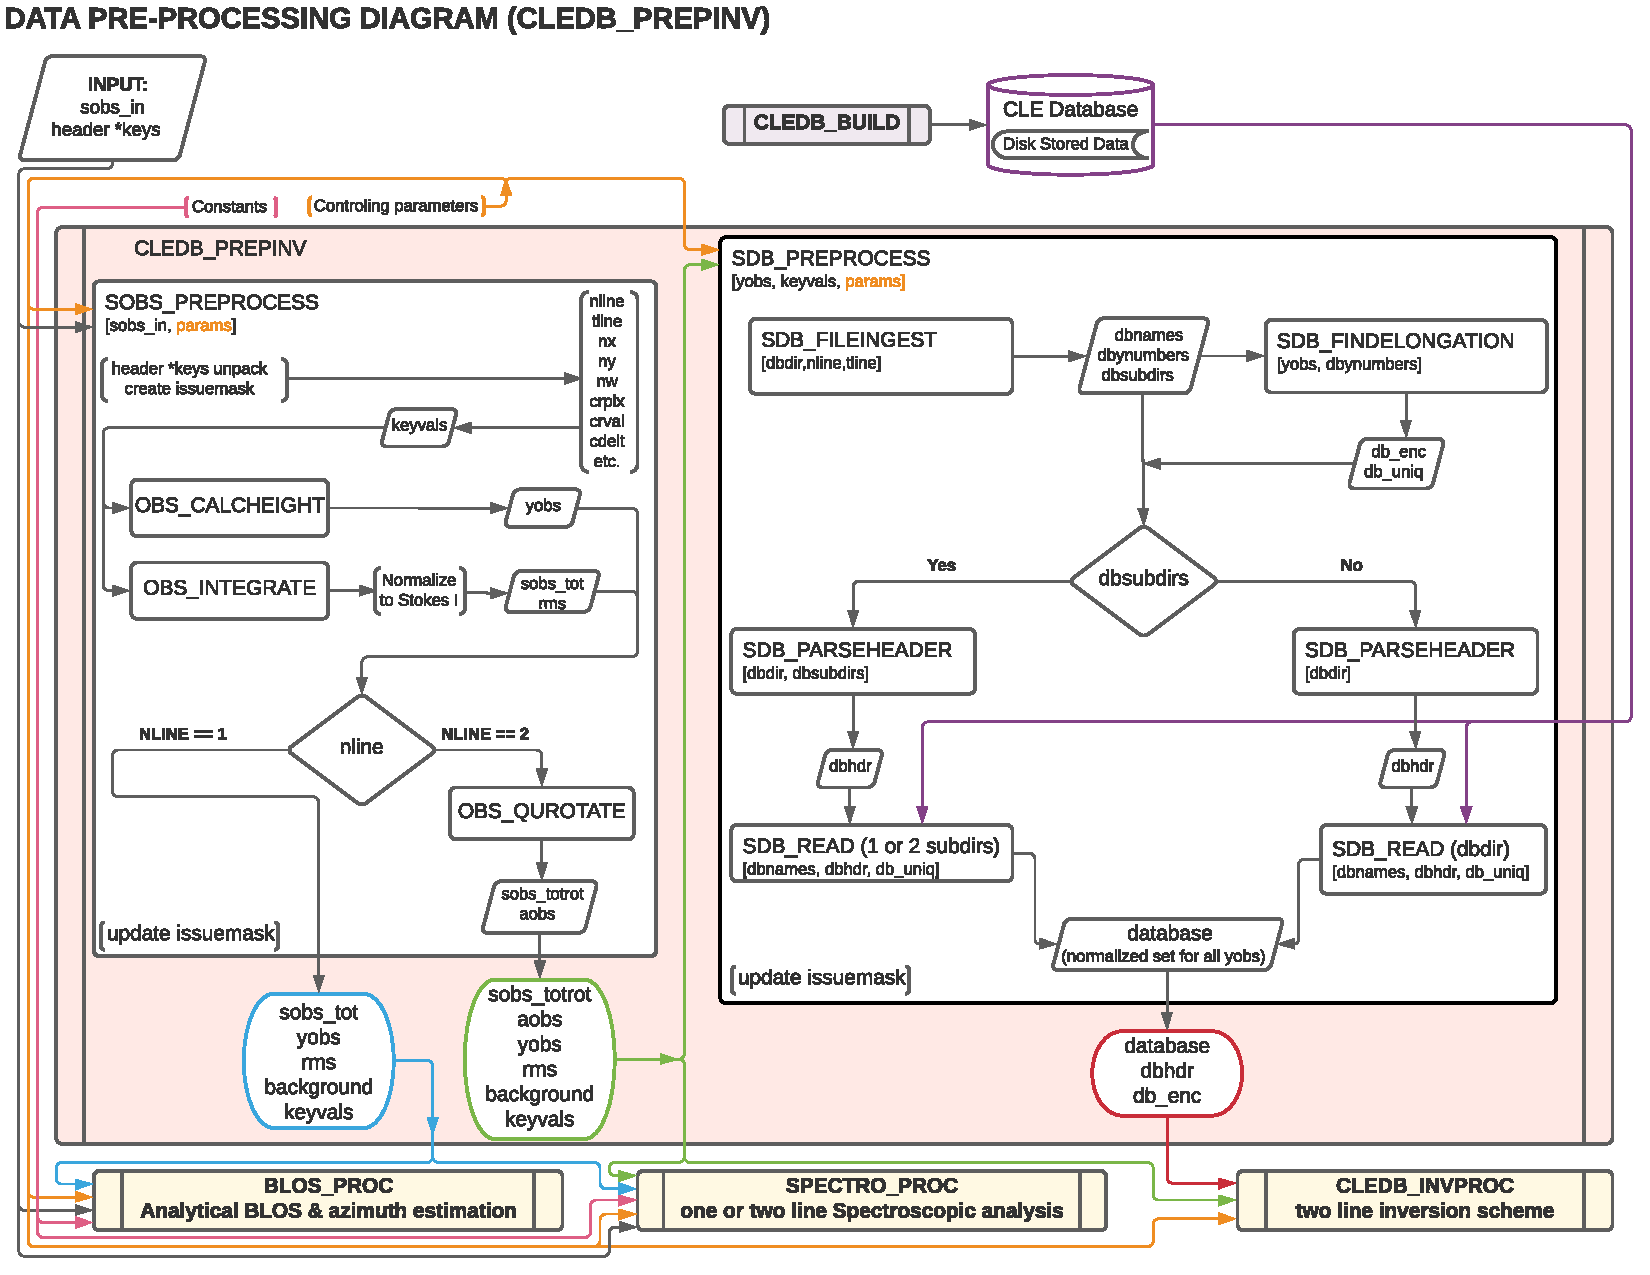
\includegraphics[angle=-90,width=1.12\columnwidth]{figs/3_CLEDB_PREP.pdf}
\end{figure} 

\newpage

\textbf{CLEDB\_PREPINV main variables:}
\begin{description}
    [font=\normalfont,leftmargin=1.3in,style=multiline]
    \item[sobs\_tot]
        [xs,ys,nline*4] float array; It contains the background subtracted, integrated, and normalized Stokes IQUV spectra. 
    \item[sobs\_totrot]
        [xs,ys,nline*4] float array; It is derived from sobs\_tot, where the QU components are rotated along the center of the Sun to match the reference direction for linear polarization (the reference in which the database is created by CLEDB\_BUILD). In inner functions of CLEDB\_PROC only 1 pixel is passed at a time as sobs\_1pix. The variable is initialized as a "zero" array that is returned in the case of 1-line observations to keep a standardized function input/output needed for vectorization.        
    \item[background]
    	   [xs,ys,nline*4] float array; returns averaged background counts for each voxel and each stokes component. 
    \item[rms]
       [xs,ys,nline*4] float array; returns the root mean square (rms) of the total counts in each Stokes profile. The rms calculation is correspondent to the ratio between intensity in the line core and background counts (the variance). This measurement shows the quality in the signal for a particular voxel.         
    \item[yobs]
       [xs,ys] float array; the header keyword input is used to construct a height projection for each observed voxel in units or $R_\odot$. In inner functions of CLEDB\_PROC only 1 pixel is passed at a time as yobs\_1pix.
    \item[aobs]
       [xs,ys] float array; it contains the linear polarization angle transformation performed by the OBS\_QUROTATE function. This information is used to derotate the matched database profiles found by the CLEDB\_INVPROC 2-line inversion module. In inner functions of CLEDB\_PROC only 1 pixel is passed at a time as aobs\_1pix. The variable is initialized as a "zero" array that is returned in the case of 1-line observations.
    \item[dbsubdirs]
       string or string list; contains the directory structure formatted as described in the CLEDB\_BUILD output section.
     \item[database]
        list of [ned,nx,nbphi,nbtheta,nline*4] float arrays; The list is the minimal subset of databases that are compatible with the observation taking to account the ny resolution of the database.        
     \item[dbhdr]
        list of ints, floats and strings; Database header information containing the parameters used to generate the database.  
     \item[db\_enc]
        [xs,ys] float array; keeps an encoding of which of the memory loaded databases to use for matching in each voxel.          
    \item[issuemask]
        [xs,ys] float array; an array that encodes issues appearing during processing of all modules. The issuemask is described separately below.        
      \item[Note:]
       Input variables, e.g. header *keys, sobs\_in, ctrlparams, constants, etc. that are described in the section above are not repeated here.                                  
\end{description}


\newpage
\subsection*{\Large CLEDB\_PROC Data Analysis \& Inversion}

\textbf{Purpose:} Three modules, SPECTRO\_PROC, BLOS\_PROC, and CLEDB\_INVPROC are grouped under the data analysis and inversion section. Based on the one or two line input data, two of the three modules are called. Line of sight or full vector magnetic field outputs along with plasma, geometric and spectroscopic outputs are inverted here. The algorithm flow and a processing overview is described in the below diagram. 

~

\textbf{A. SPECTRO\_PROC module}

\textbf{Purpose:} Ingests the full spectroscopic prepped data (from OBS\_PREPROCESS) and produces spectroscopic outputs for each input line. Part of the outputs are used downstream in BLOS\_PROC or CLEDB\_INVPROC. This module is heavily dependent on the CLEDB\_PREPINV processing.  Optional sub-modules are envisioned to be integrated into this processing based on upstream instrument processing and retrieved data quality.

~

\textbf{SPECTRO\_PROC main functions:}
\begin{description}
    [font=\normalfont,leftmargin=2.1in,style=multiline]
    \item[CDF\_STATISTICS]
        Performs analysis on the stokes IQUV spectra for each line and computes relevant spectroscopic outputs (see variable description below) by using a non-parametric approach, the analysis of cumulative normal distribution functions.
    \item[(Opt.) ML\_LOSDISENTANGLE]
        To be implemented at a later time. Uses Machine learning techniques for population distributions to disentangle multiple emitting structures along the LOS.
    \item[(Opt.) LEV2CALIB\_WAVE]
        To be implemented at a later time. Higher order wavelength calibration using the spectroscopic profiles. See \citet{Ali+2021} for additional details. This function can couple if the upstream wavelength accuracy of the input observation is missing or is less than 0.01nm.
    \item[(Opt.) LEV2CALIB\_ABSINT]
        To be implemented at a later time, if feasible. Absolute intensity calibration function that produces an additional output, the calibrated intensity in physical units. The approach is not easily automated as it requires a more convoluted and specific planning of the observations to gather the necessary input data.                        
\end{description}

~

\textbf{SPECTRO\_PROC main variables:}
\begin{description}
    [font=\normalfont,leftmargin=1.3in,style=multiline]

    \item[(opt.) sobs\_cal]
        [nx,ny,sn,4] array; optional calibrated level-2 data in intensity and or wavelength units. This is then used by the CDF\_STATISTICS function instead of sobs\_in.                 	
        \item[specout]
		[nx,ny,nline,12] (output)float array; returns the 12 available spectroscopic output calculations, for each input line, and for every pixel location.

		 
    \item[]
    		specout[:, :, :, 0]; Wavelength position of the line core; nm units.
    \item[]
    		specout[:, :, :, 1]; Doppler shift with respect to the theoretical line core; nm units.
    \item[]
        specout[:, :, :, 2]; Doppler shift with respect to the theoretical line core; km s$^{-1}$ units.
    \item[]
    		specout[:, :, :, 3:7]; Intensity at line center wavelength for Stokes I, Q, and U. Stokes V intensity is given as the maximum or minimum counts in the core of the first (left) lobe. Thus, the Stokes V intensity measurement will not match the wavelength position of the Stokes IQU intensities; ADU units or calibrated physical units if LEV2CALIB\_ABSINT is utilized.)
    \item[]
    		specout[:, :, :, 7]; Averaged background intensity outside the line profile for the Stokes I component. Since background counts are independent of the Stokes measurement, we utilize just this one realization; ADU units or calibrated physical units if LEV2CALIB\_ABSINT is used.)
    \item[]
    		specout[:, :, :, 8]; Total line full width at half maximum (FWHM); nm units.
    \item[]
    		specout[:, :, :, 9]; Non-thermal component of the line width. A measure or estimation of the instrumental line broadening/width will significantly increase the accuracy of this determination; nm units.

    \item[pl]
    		specout[:, :, :, 10]; Fraction of linear polarization with respect to the total intensity; dimensionless.                              
    \item[pv]
    		specout[:, :, :, 11];  Fraction of total polarization (linear+circular) with respect to the total intensity; dimensionless.
	\item[Note:]
		Regardless if solving for 1-line or 2-line observations, specout will return two nline dimensions. In the case of 1-line observations, the dimension corresponding to the second line remains just 0 all throughout. The unused dimension can be removed from the upstream script, if needed. This behavior is known and enforced to keep output casting static, speeding up execution when using numba.
\end{description}

~

~

\textbf{B. BLOS\_PROC module}

\textbf{Purpose:} Implements analytical approximations of \citet{1999ApJ...522..524C} and \citet{2020ApJ...889..109D} to calculate the LOS projected magnetic field strength and magnetic azimuth angle. The module returns two degenerate constrained magnetograph solutions, where the one that matches the sign of the atomic alignment is very precise, along with the less precise "classic" magnetograph formulation.

 This branch is activated for 1-line observations (4 stokes profiles) where the problem is too underdetermined to apply the full inversion database approach using the CLEDB\_INVPROC module.

\textbf{BLOS\_PROC main variables:}
\begin{description}
    [font=\normalfont,leftmargin=1.1in,style=multiline]
    \item[blosout]
        [nx,ny,4] (output) array; line of sight projected magnetic field estimations and magnetic azimuth angle; G units.
    \item[]        
        blosout[:, :, 0] First degenerate constrained magnetograph solution. 
    \item[]         
        blosout[:, :, 1] Second degenerate constrained magnetograph solution.
    \item[]         
        blosout[:, :, 2] "Classic" magnetograph solution. Precision is the average of the two above degenerate solutions. 
    \item[]
        blosout[:, :, 3] Magnetic field azimuth angle derived from the Q and U linear polarization components; Because of using arctan functions to derive, there is a $/pi/2$ degeneracy manifesting in a map.\\ -$\pi$ to $\pi$ range.
    \item[Note:]
    The "classic" magnetograph estimation is less precise than the optimal degenerate constrained magnetograph solution, but more precise than the other. Using just the 4 Stokes IQUV of one observation does not allow us to disentangle which of the two constrained magnetograph solutions is optimal.
                    
\end{description}


\begin{figure}[!p]
\vspace{-1cm}\hspace{-1.2cm}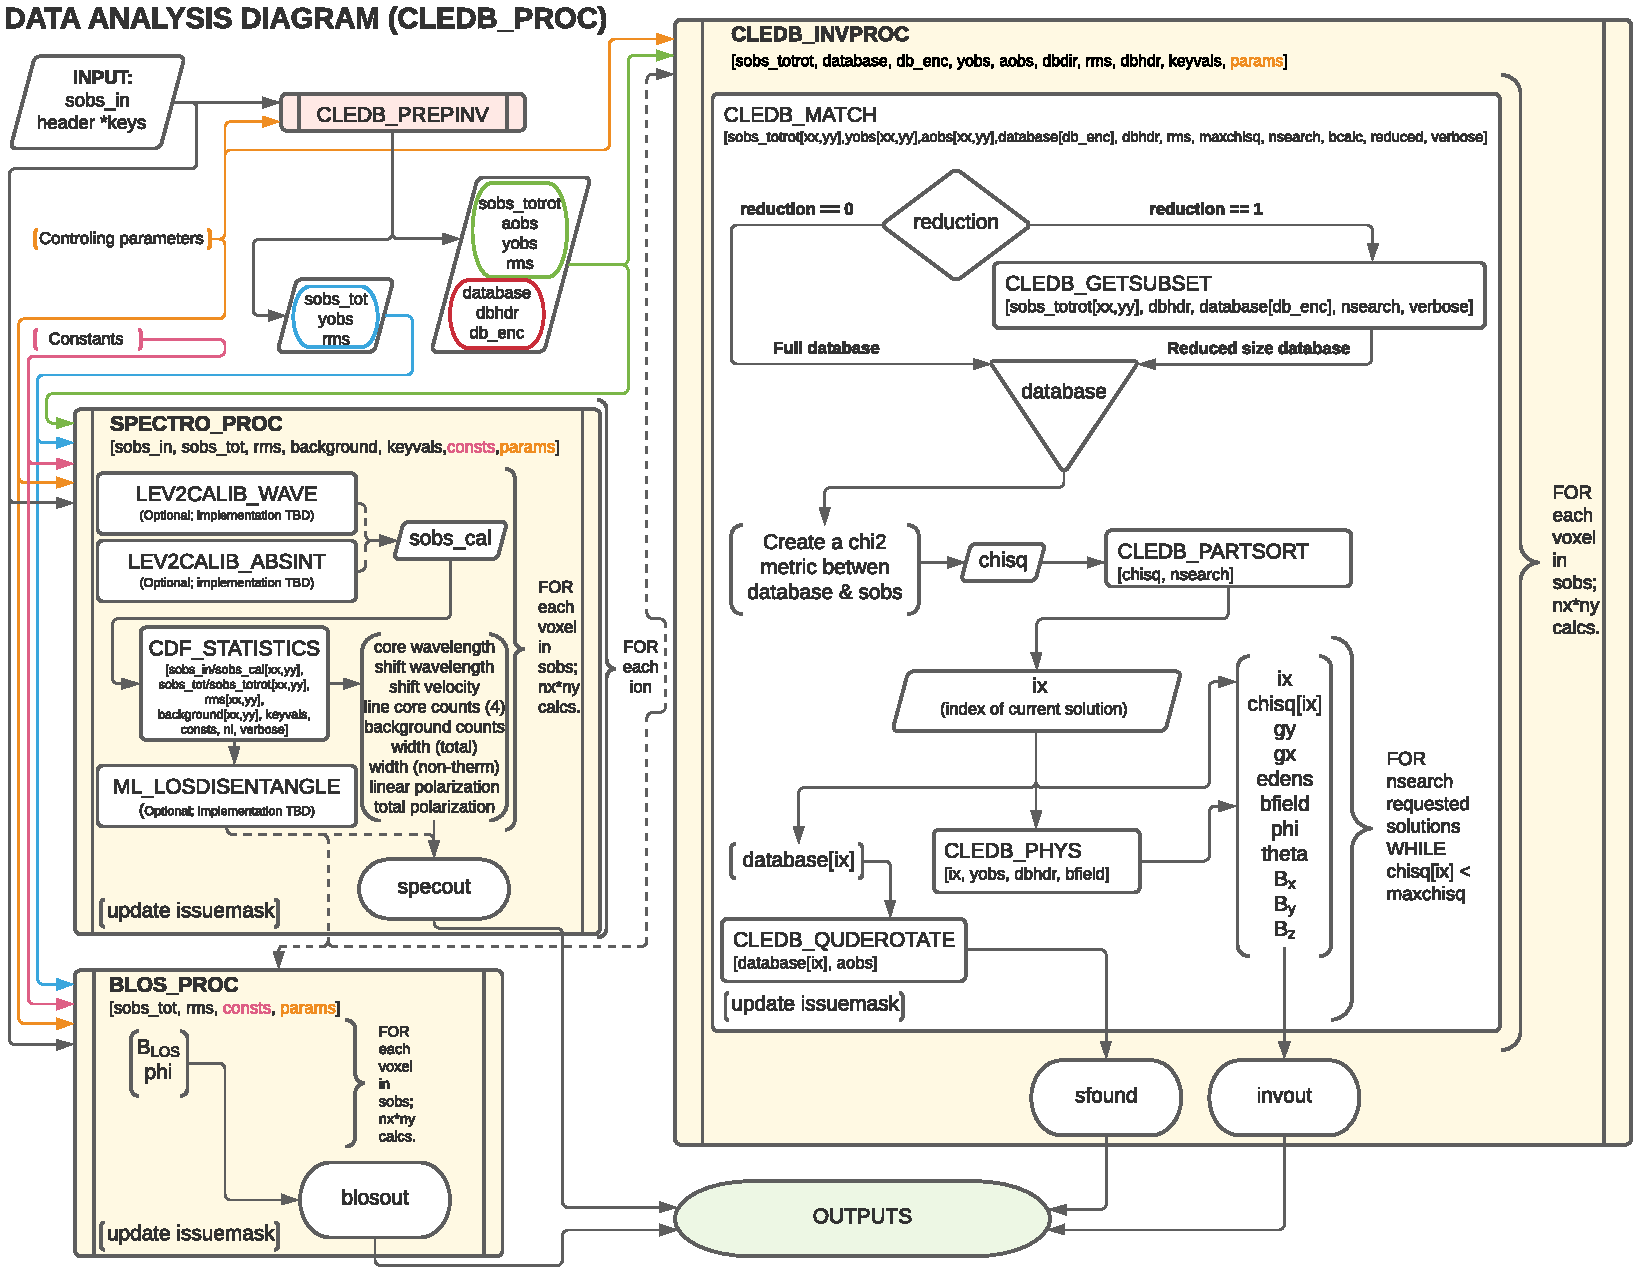
\includegraphics[angle=-90,width=1.12\columnwidth]{figs/4_CLEDB_PROC.pdf}
\end{figure} 

\newpage

\textbf{C. CLEDB\_INVPROC module}

\textbf{Purpose:} Main inversion module. CLEDB\_INVPROC compares the preprocessed observations with the selected databases by performing a $\chi^2$ goodness of fit measurement between each independent voxel and the complete set of calculations in the matched database. If CLEDB\_GETSUBSET is utilized, a presorting of the database entries to those that match the direction of lienar polarization is performed. This might presorting might slightly change the final ordering of solutions in certain cases, where some apparently compatible solutions are removed. After the main sorting is performed, the best database solutions are then queried with respect to the physical parameters that gave the matched profiles. 

~

\textbf{CLEDB\_INVPROC main functions:}
\begin{description}
    [font=\normalfont,leftmargin=1.8in,style=multiline]
	\item[CLEDB\_MATCH]
		Matches a set of two full Stokes IQUV observations with a model observation  of the same Stokeq quantities. Matching is done individually for each requested pixel in the input array. This is the most time-consuming function. runtime estimations are provided below.  
    \item[$\Dsh$ CLEDB\_GETSUBSET]
        When enabled, the information encoded in the azimuth is used to reduce the matched database by approximately 1 order of magnitude in terms of calculations. If this subset calculation is disabled from the ctrlparams, execution time in the case of large databases is significantly increased. Although small differences between full and subset sorted database solutions exist, our synthetic data tests did not reveal a situation where performing a calculation with the full database returned a better matching result.  
    \item[$\Dsh$ CLEDB\_PARTSORT]
		A manual function that performs only a partial sort of the array because only a small subset of solutions are usually returned. This increases execution times by a few factors when requesting just few solutions (<50 on 10$^8$ entries databases). The partial sort function is used by both CLEDB\_MATCH and CLEDB\_GETSUBSET functions. In CLEDB\_MATCH, CLEDB\_PARTSORT performs a manual sorting of database entries based on the $\chi^2$ metric. Utilized in CLEDB\_GETSUBSET, CLEDB\_PARTSORT selects for each $\phi$ angle orientation only the most compatible $\Theta$ directions based on the azimuth given by the linear polarization measurements.
    \item[$\Dsh$ CLEDB\_PHYS]
        Returns 9 physical and geometrical parameters corresponding to each selected database index inside the nsearch and maxchisq constraints. these are described below.
    \item[$\Dsh$ CLEDB\_QUDEROTATE]
        Derotates the Q and U components from each selected database entry, in order to make the set of measurements comparable with the original integrated input observation                        
\end{description}

~

\textbf{CLEDB\_INVPROC main variables:}
\begin{description}
    [font=\normalfont,leftmargin=1.3in,style=multiline]
    \item[database]
        list of [ned,nx,nbphi,nbtheta,nline*4] float arrays at input; Individual voxel indexes of the list variables are fed to the CLEDB\_MATCH module. From the database list, only the best matching height entry via db\_enc is passed to CLEDB\_MATCH via database\_sel internal variable. 
	\item[database\_sel]  
        Subset index of the database list that is fed to CLEDB\_MATCH for matching the observation in one voxel. This eases memory shuffling and array slicing operations. This array is reshaped into a 2D  [ned*nx*nbphi*nbtheta(index),nline*4] form. In the case where reduction is selected, the variable is additionally reduced with respect to the number of potential indexes to match. 
    \item[chisq]
        [ned*nx*nbphi*nbtheta,nline*4] float array; Computes the squared difference between the voxel [nline*4] IQUV measurements and each index element of the database [index,nline*4].
    \item[sfound]
        [nx,ny,nsearch,nline*4] (output) float array; returns the de-rotated and matched nsearch IQUV*nline solutions of the database.
        
\newpage           
    \item[invout]
    		[nx,ny,nsearch,11] (output) float array; Main two-line inversion output product. invout contains the matched database index, the $\chi^2$ fitting residuals, and 9 inverted physical parameters, for all nsearch closest matching solutions with respect to the input observation. The 11 parameters follow with individual descriptions.
    	\item[]  
    		invout[nx,ny,nsearch,0] - index; The index of the database entry that was matched at the nsearch rank. The index is used to retrieve the physics that match the observations. 
    	\item[]  
    		invout[nx,ny,nsearch,1] - chisq; The $\chi^2$ residual of the matched database entry.
    	\item[]  
    	    invout[nx,ny,nsearch,2] - edens; Plasma density computed via the ratio of the two ions inverted. This output is applicable for the Fe XIII 1074.68/1079.79 line ratio (same ion). Other line combinations will produce less accurate results due to the relative abundance ratios, that are varying dynamically. For a real-life observation, we do not consider trustworthy the implicit static relative abundance ratios of different ions, resulted from the CHIANTI base tabular data ingested from the ATOM files to build databases. Units are logarithm of number electron density in cm$^{-3}$.
    	\item[]   
    		invout[nx,ny,nsearch,3] - gy; observation apparent height; analogous to yobs variable; $R_\odot$ units.
    	\item[]
    		invout[nx,ny,nsearch,4] - gx; Position of the dominant emitting plasma along the LOS; $R_\odot$ units. 
    	\item[]
    		invout[nx,ny,nsearch,5] - bfield; Magnetic field strength recovered via the ratio of observed stokes V to database Stokes V (computed for B = 1 G); Uses bcalc control parameter; G units.       	
    	\item[]  
    		invout[nx,ny,nsearch,6] - bphi; Magnetic field azimuth angle; 0 to $2\pi$ range.
    	\item[]
    		invout[nx,ny,nsearch,7] - btheta; Magnetic field LOS angle; 0 to $\pi$ range.      	
    	\item[]
    		invout[nx,ny,nsearch,8] - bx; Cartesian projected magnetic field depth/LOS component; G units.
    	\item[]
    		invout[nx,ny,nsearch,9] - by; Cartesian projected magnetic field horizontal component; G units.  	
    	\item[]
    		invout[nx,ny,nsearch,10] - bz; Cartesian projected magnetic field vertical component; G units.
    	\item[Note:]
    	   Regardless of the number of solutions (if any) that are found, the outinv array will return  "0" value arrays, with only the index set to "-1" to keep output data shapes consistent. 	                       
\end{description}


\newpage
\subsection*{Outputs}

The main CLEDB inversion algorithm outputs are stored in the following variables:
\begin{description}
    [font=\normalfont,leftmargin=1.2in,style=multiline]
\item[$\qquad\bullet$ \textbf{specout}] 
 12 SPECTRO\_PROC output products.
\item[$\qquad\bullet$ \textbf{blosout}]  
4 BLOS\_PROC output products.
\item[$\qquad\bullet$ \textbf{invout}]  
11 CLEDB\_INVPROC output products.
\item[$\qquad\bullet$ \textbf{issuemask}]  
Records any issues that arisex in processing for each voxel (to be implemented).
\end{description}
The three main output products are listed in the simplified module scheme. The individual products are described in the "main variable" lists of the three data analysis \& inversion modules.

~

\textbf{Tentative issuemask implementation}

The inversion will implement a confidence/issue map [nx,ny] for all spatial pixels in an input observation that will be returned along with the main output products. 

Note: Issuemask encoding not currently active. Final form to be decided and implemented. 

~

\textbf{Example of issuemask coding:}
\begin{description}
    [font=\normalfont,leftmargin=0.6in,style=multiline]
    \item[0]
        No apparent problem in voxel.
    \item[1]
        One or more of Stokes I, Q, U are lower than noise RMS threshold.
    \item[2]
        Stokes V is lower than noise RMS threshold.
    \item[4]
        Linear polarization is close to Van-Vleck ambiguity (warning).  
    \item[8]
        B$_{LOS}$ or $\phi$ is lower than noise threshold (for 1-line obs).
    \item[16]
        Database fit failed to converge reliably (for 2-line obs).
    \item[32]
        One or more of B, phi, theta are lower than noise threshold (for 2-line observations).
    \item[64]
    ..........      
    \item[128]
    ..........               
\end{description}
Coding the information sequentially when processing through the different module, will be done by using powers of 2. The issuemask values are thus cumulative. Following the example of the confidence map coding from above, we define for example a pixel from a 1-line observation with unreliable Stokes V signal. The uncertainty in Stokes V will also lead to compromised B$_{LOS}$ information. Thus, the issuemask will encode a value of 10 for that respective pixel.


\newpage

\subsubsection*{Execution timing examples}



 \begin{figure}[!h]
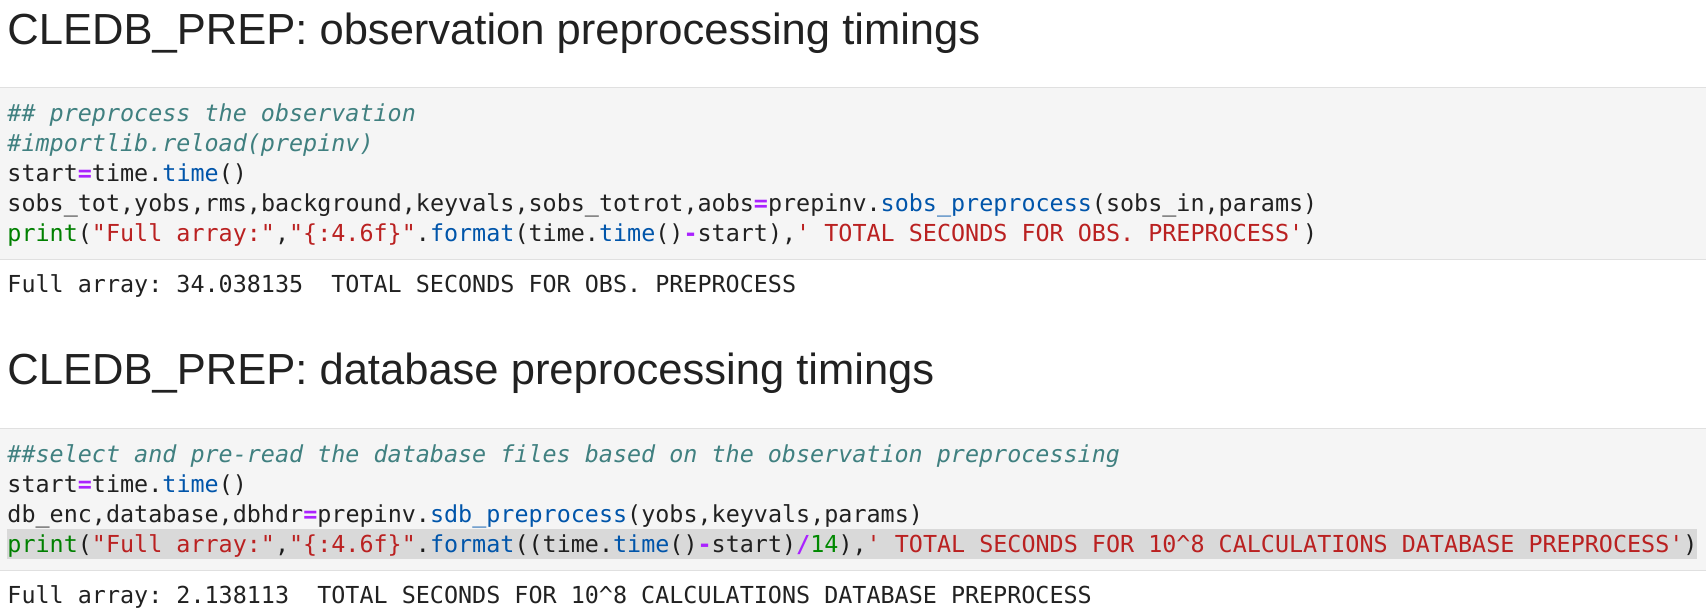
\includegraphics[width=0.75\columnwidth]{figs/calc_time_prep.png}
\caption*{Timing of the full test array execution for a 2-line observation and database preprocessing. Timing division for database preprocessing comes from loading 14 databases into memory.}
\end{figure} 

 \begin{figure}[!h]
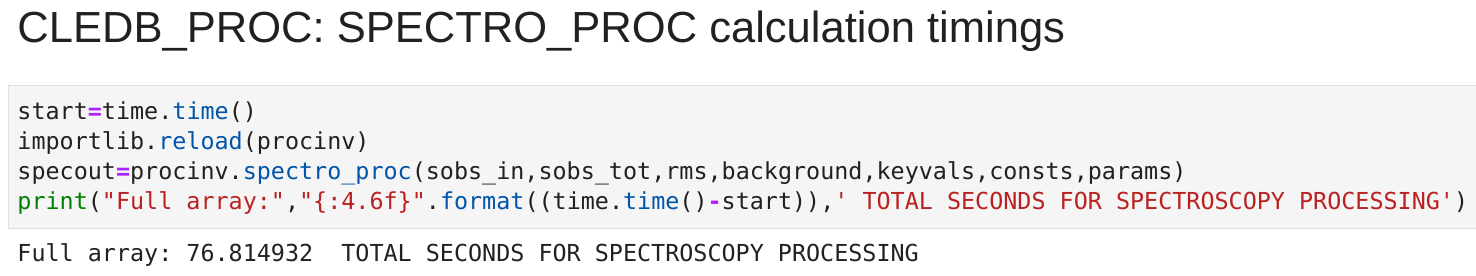
\includegraphics[width=0.65\columnwidth]{figs/calc_time_spectro.png}
\caption*{Timing of the full test array execution for a 2-line observation spectroscopic processing.~~~~~~~~~~~~~~~~~~~~~~~~~~~~~~~~~~~~~~~}
\end{figure} 

 \begin{figure}[!h]
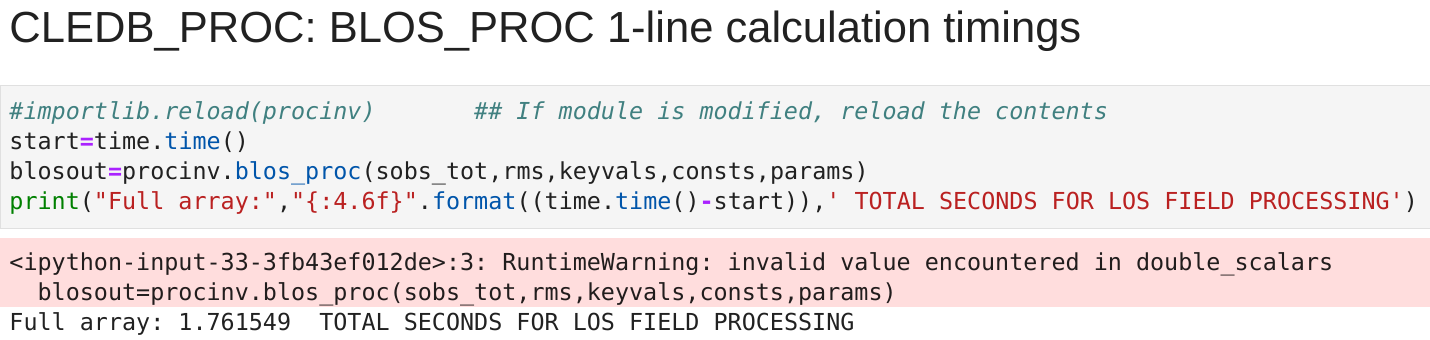
\includegraphics[width=0.65\columnwidth]{figs/calc_time_blos.png}
\caption*{Timing of the full test array execution for a 1-line observation line of sight magnetic field processing.~~~~~~~~~~~~~~~~~~~~~~~~~~~~~~~~~~~~~}

\end{figure} 
 \begin{figure}[!h]
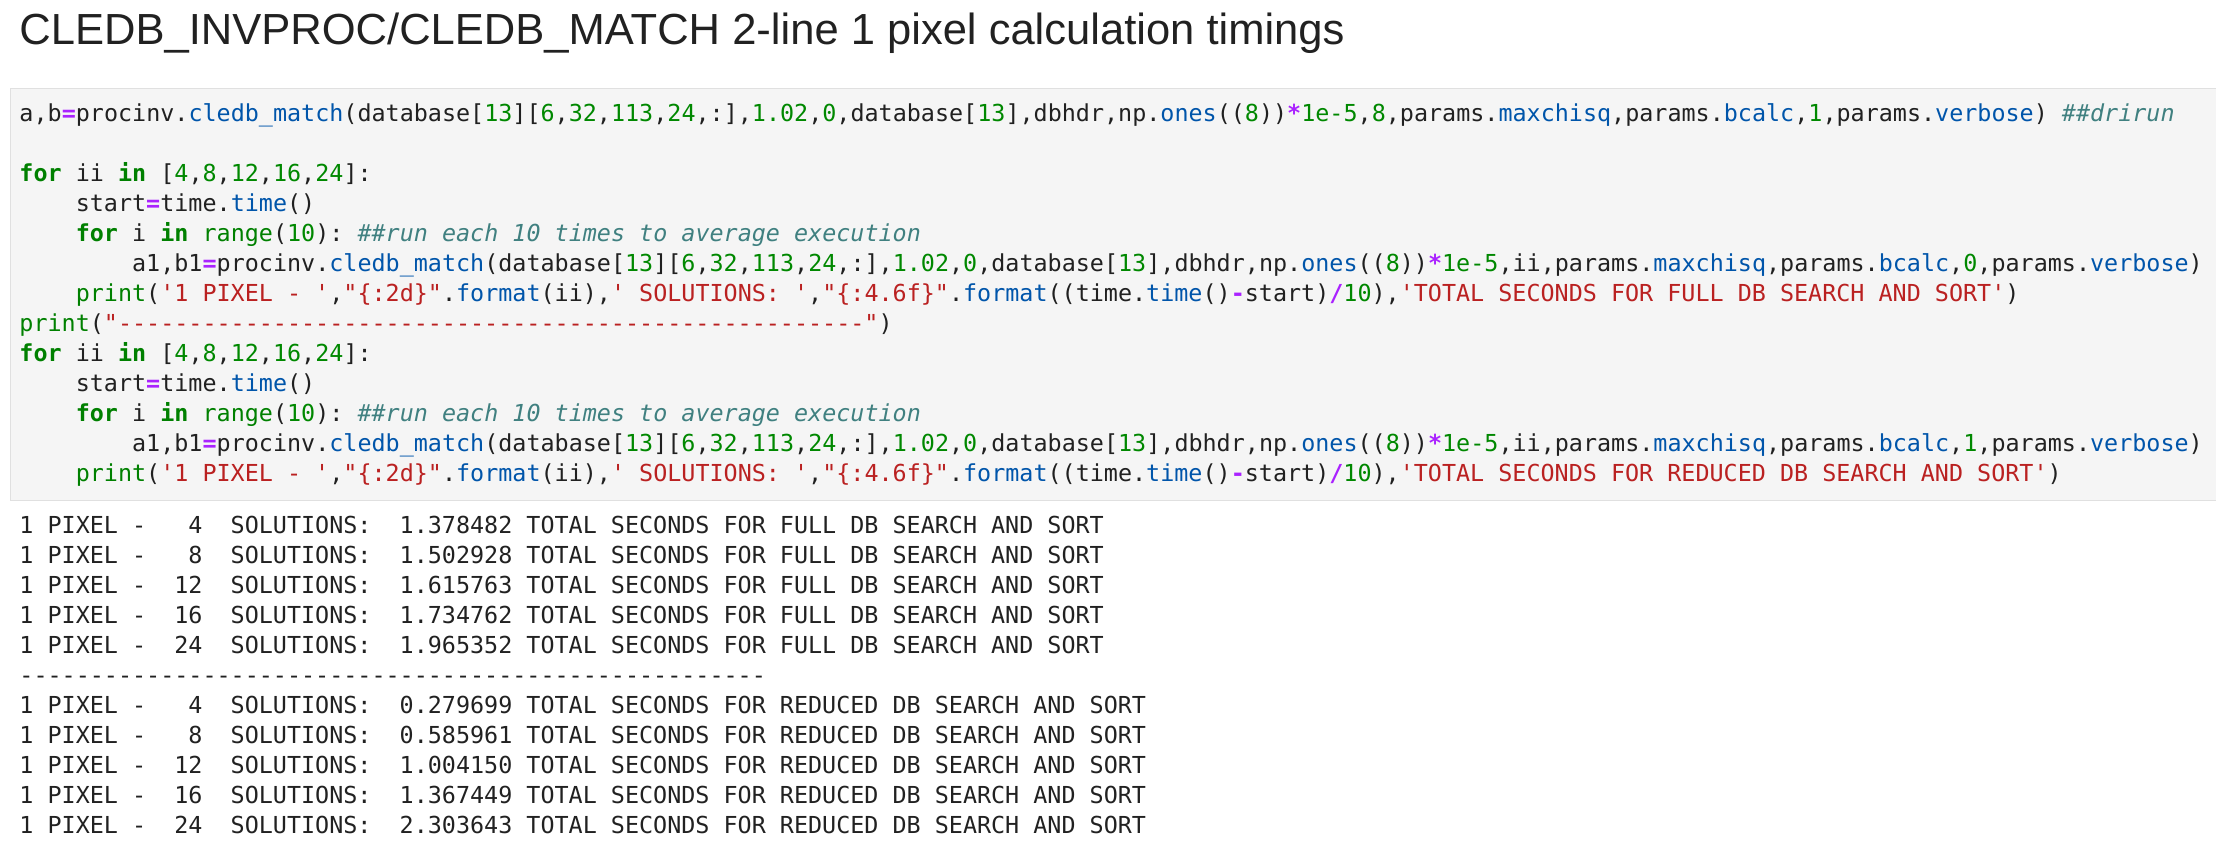
\includegraphics[width=0.85\columnwidth]{figs/calc_time_1pix.png}
\caption*{Timing of the single thread execution for a 2-line magnetic field inversion of a single point (1 pixel) observation. Multiple runs are produced to average timings. Due to the resource intensive task to be queried, this timing is different from previous modules!}
\end{figure} 

CLEDB\_INVPROC is the most time consuming part of the CLEDB algorithm. A single laptop CPU thread implementation applied to a 1024 by 1024 array will run for 15+ hours. Numba parallelization scales with available resources, potentially making computations near instant on a research computing system.  

\newpage

\subsubsection*{Terminology glossary} 

\begin{description}
    [font=\normalfont,leftmargin=1.3in,style=multiline]
    \item[ADU]
    Arbitrary Data Units; detector calibrated counts when no absolute intensity calibration exists.
    \item[Analytical solution]
        frame an inverse problem in a well-understood mathematical form and  approximates a solution. 
    \item[CDF]
    		Cumulative Distribution Function. Statistical method for interpreting normal distributions. 
    \item[CLE \& CLEDB]
		Coronal Line Emission DataBase FORTRAN spectral synthesis code variants.
	\item[CHIANTI]
	atomic database for spectroscopic diagnostics of astrophysical plasmas; documentation \href{https://www.chiantidatabase.org/}{available}.
    \item[$\chi^2$ fitting solution]
        Statistical hypothesis to determine whether a variable is likely to come from a specified distribution. The $\chi^2$ residual is used to find the closest match to a discrete distribution point. 
    \item[Degeneracy]
        When performing an inversion, the degrees of freedom of the problem might not allow to recover an exact mathematical solution. Sets of equivalent solutions inside an inversion metric are called degenerate. e.g., disentangling an angle value knowing that $\sin a =\frac{1}{2}$; a is degenerate to $\frac{\pi}{6}$ or $\frac{5\pi}{6}$	
	\item[FWHM]
	Full Width at Half Maximum. Measurement of a standard width of a normal distribution.    
    \item[header (input file)]
        sets of metadata that accompanies an observation datafile.
    \item[Inversion]
        mathematical process that starts from the output of a physical 		process and backtraces to recover one or more input variables. In our particular case, we start from output Stokes IQUV profiles and attempt at recovering coronal magnetic fields responsible for producing said profiles.
	\item[JIT]
	Just In Time compilation decorator from the Numba library package.
    \item[LOS]
    		Line Of Sight.
    	\item[Normal distribution]
    	A Gaussian function, or a bell curve. Probability distribution that is symmetric around a mean value, in which data near the mean are more frequent in occurrence than data far from the mean. 
    	\item[Numba]
    	An open source JIT compiler that translates a subset of Python and NumPy code into fast machine code. Serial task parallelization is also available.
    	\item[Numpy]
    Open source library for fast numeric operations.	
    \item[Physical units]
        Definition of measurement that is calibrated to physically etalonated constants;\\ e.g. intensity in [erg cm$^{-2}$ s$^{-1}$ $\AA^{-1}$ sr$^{-1}$]
    \item[Radiative transfer]
        Transfer of electromagnetic radiation through a medium.
    \item[Stokes parameters] 
        A set of values or spectra that describe the polarization state of electromagnetic radiation.       
    \item[Spectroscopic data] 
       Electromagnetic radiation flux spread in individual bins inside an electromagnetic spectral range.
    \item[Spectroscopic emission line]
        Excess flux exceeding background counts at determined spectral positions, occurring when the electrons of an excited atom or molecule move between energy levels.  
    \item[Stokes I]
        Total intensity of spectroscopic line emission.
    \item[Stokes Q \& U]
        Linear polarization components of spectroscopic line emission.
    \item[Stokes V]
        Circular polarization component of spectroscopic line emission.
    \item[Voxel]
        A generalized concept of a pixel. In our case, by voxel we envision 2D projection of a volume inside a square area that contains information about the integral along the line of sight.                     
\end{description}

\vfill

{\scriptsize\bibliography{refs.bib} }
\end{document}
